\def\itk{KiSD}
\def\pm{PBSM}
\chapter{实验设计与结果分析}
\label{ch5:experiment}
\section{实验设置}
本章主要介绍了实验的设置与设计。首先我们介绍了实验的软硬件平台环境以及数据集来源和评价标准,
其次,阐述了查询图的生成方法,具体包括从数据图中随机提取子图的方式及不同查询图大小的设置。
接着,我们介绍了实验中使用的不同算法对比,包括本文所有提出的优化算法、多种现有的连续子图匹配算法以及两种静态的top-k算法。
\subsection{实验环境}
本节对我们提出的解决方案进行了评估。
所有方法均采用C++实现,并在配置为64GB内存、Intel(R) 4210R CPU @ 2.40GHz的CentOS服务器上运行。
实验所用的所有代码和数据集可在GitHub上获取~\cite{code-git-csmtok}。
实验所依赖软硬件操作平台配置如表\ref{table:setup}所示。
\begin{table}[H]
    \centering
    \caption{实验环境配置}
    \label{table:setup}
    \begin{tabular}{cc}
        \toprule
        描述   & 型号  \\
        \midrule
        CPU处理器 & Intel(R) 4210R CPU @ 2.40GHz\\
        内存 & 64G \\
        硬盘 & 1T\\
        操作系统 & CentOS Linux 7 (Core)\\
        编程语言 & C++ \\
        \bottomrule
    \end{tabular}
\end{table}

\subsection{数据集和评价标准}
\label{ss-sec:dataset}
在本实验中,我们参考了之前关于CSM(Subgraph Matching)的研究工作~\cite{csm-survey:DBLP:journals/pvldb/SunSLH22,static-sm:DBLP:conf/sigmod/Sun020},并选择了五个广泛使用的真实数据集进行实验。
这些数据集代表了不同领域的图数据,包括社交网络、电子商务、蛋白质相互作用网络等,能够涵盖多种不同的数据分布特征,并为评估算法的性能提供丰富的测试场景。具体数据集如下:
\begin{itemize}
\item Amazon 数据集:该数据集来源于亚马逊网站,包含了一个产品购买网络图,反映了用户之间的购买行为和偏好。
\item LiveJournal 数据集:这是一个社交网络数据集,包含了来自LiveJournal平台的社区网络,具有较为复杂的社交结构。
\item Human 数据集:该数据集包含了一个蛋白质相互作用网络图,广泛用于生物信息学研究,能够反映蛋白质之间的相互作用关系。
\item YouTube 数据集:该数据集来源于YouTube平台,包含了用户之间的社交关系网络图,常用于社交网络分析。
\item Orkut 数据集:这是一个免费开放的在线社交网络数据集,它允许用户搭建好友关系,分享各类内容,数据集涵盖了广泛的社交互动数据。
\end{itemize}   

具体测试的数据集规模如表\ref{table:dataset}所示,表中列出了每个数据集的顶点数($|V|$),边数($|E|$),顶点标签数($|L(V)|$),边标签数($|L(E)|$),以及图的平均度($degr(G)=\frac{2|E|}{|V|}$)。
这些数据集的顶点数从 4 千到 307 万不等,边数从 8 万到 1.17 亿,基本覆盖了现实世界中常见的图数据规模,能够有效反映算法在不同规模下的处理能力与适应性。通过在上述数据集上的系统性实验评估,我们可以全面验证本文提出方案在时间效率与空间开销方面的综合性能,从而展示其在大规模动态图处理中的扩展性和稳定性。

\begin{table}[H]
    \centering
    \caption{数据集信息描述}
    \label{table:dataset}
    \begin{tabular}{cccccc}
        \toprule
        数据集   & $|V|$  & $|E|$ & $|L(V)|$ & $ |L(E)|$ & $degr(G)=\dfrac{2|E|}{|V|}$\\
        \midrule
        Amazon    & 403,394 & 1,015,000 & 6 & 1 & 5.03     \\ 
        LiveJournal   & 4,847,571 & 30,005,000 & 30 & 1 & 12.38 \\ 
        Human  & 4,674 & 81,282  & 44 & 1 & 34.78   \\ 
        YouTube  & 1,134,890 & 2,015,000 & 25 & 1 & 3.55  \\ 
        Orkut  & 3,072,441 & 117,185,083 & 10 & 1 & 76.28  \\ 
        \bottomrule
    \end{tabular}
\end{table}

请注意,以上数据集中的边均为无权边。对于每条边 $(v_1, v_2)$,我们为其分配一个权重,计算方式为:
\begin{equation}
    \frac{(N(v_1) \cap N(v_2)) + 1}{(N(v_1) \cup N(v_2)) + 1}
\end{equation}
其中,$N(v_1)$ 和 $N(v_2)$ 分别表示顶点 $v_1$ 和 $v_2$ 的邻居节点集合,计算结果保留六位小数。
这个方法通过衡量两个顶点的邻域交集与并集的比值,反映了它们之间的连接强度(+1是为了防止出现分母为0的情况)。
对于上述数据集,我们通过从每个图中随机抽取 $10,000$ 条边来构建相应的更新流。
这些更新流用于模拟实际应用中频繁的图更新操作。
通过这些实验设置,我们能够全面评估所提出的算法在不同规模图数据上的表现,尤其是在大规模数据集中的时间和空间效率。


\textbf{查询图生成}
\label{ss-sec:querygen}

与之前的研究~\cite{csm-turboflux-DBLP:conf/sigmod/KimSHLHCSJ18,csm-symbi-DBLP:journals/pvldb/MinPPGIH21,csm-survey:DBLP:journals/pvldb/SunSLH22}类似,
我们采用从数据图中随机提取子图的方式来生成查询图。
具体地,对于每个数据集,我们设置了六种不同的查询大小 ($|E_Q|$):$6$、$8$、$10$、$12$和$14$。
对于每个查询大小,我们提取了10个查询图。
这些查询图的大小反映了实际应用中可能遇到的子图匹配问题规模。通过对这些查询图进行处理,我们能够评估不同规模查询图下算法的性能表现。对于每个查询图,
我们分别评估了不同的 $k$ 值:$100$、$300$、$500$、$700$和$900$,表示连续子图匹配中需要维护的子图匹配数量。
所有实验结果均通过对相应查询图应用不同算法,并计算结果的平均值来得出。
这样,能够确保实验结果的代表性,并减少偶然因素对实验结果的影响。
我们进一步分析了查询图的大小与算法时间、空间效率之间的关系,并通过这些实验深入评估了算法在实际应用中的表现。

\textbf{对比方法}

在本节实验中,我们将评估所提出的算法在上述真实数据集上的性能。为了全面评估我们的算法,我们将我们提出的几种优化算法进行横向对比,包括:

(1) Baseline: 第\ref{ch3:base-framework}小节中提出的CSM-TopK问题的基础计算框架,该框架利用第 $k$ 个子图匹配结果作为剪枝上限,提供了一种简单而有效的基线方案。

(2)MWstar-global:第\ref{mwstar:global}小节中提出的基于全局MWstar索引的面向CSM-TopK问题的算法。

(3)MWstar-both:第\ref{mwstar:local}小节中提出的同时基于全局MWstar和局部MWstar的索引。该算法结合了全局和局部信息,利用更紧凑的密度上限来解决CSM-TopK问题。

(4) Our-final: 第\ref{mwstar:compact-graph}小节中提出的压缩图技术,将它与局部MWstar相结合,形成我们的最终解决方案,并且作为本章实验中的对比算法。


我们将我们的最终方案Our-final(简称为Ours),与现有的具有TopK密度约束的静态子图匹配工作进行比较,包括 \itk\cite{static-topk-Gupta-DBLP:conf/icde/GuptaGYCH14} 和 \pm\cite{static-topk-Chen-DBLP:journals/ijprai/ChenLCTL18}。
此外,我们还将我们的最终方案与几种最先进的CSM方法进行了对比,包含 Graphflow\cite{csm-graphflow-DBLP:conf/sigmod/KankanamgeSMCS17}、Rapidflow\cite{csm-rapidflow-DBLP:journals/pvldb/SunSHL22} 和 CaLiG~\cite{csm-calig-DBLP:journals/pacmmod/YangZZY23}。
需要注意的是,\itk 在处理 LiveJournal、Orkut和YouTube数据集时,因内存不足而导致无法执行,相关实验结果标记为“无穷大”。

\section{实验结果分析}
\label{ch5:overall-compare}
本节详细分析了我们提出的算法在不同实验设置下的性能表现。
我们通过与现有的对比算法在多个维度上进行比较,展示了我们算法的优势。
实验结果主要集中在以下几个方面:插入与删除效率、空间效率、索引构建时间,以及不同优化策略的对比。
\subsection{插入与删除效率对比}
\label{ch5:insertion-deletion}
在这一节中,我们详细评估了所提出的算法与现有对比算法在插入与删除操作上的效率。
实验通过不同的查询图大小和参数 $k$ 值,分析了各种算法在插入和删除操作中的表现。
首先,我们通过固定参数$k$,测试查询图的大小在$6$,$8$,$10$,$12$,$14$时的插入和删除的平均时间,如图\ref{fig:time:insertion:fixQuerySize}和图\ref{fig:time:deletion:fixQuerySize}所示;
其次,我们通过固定查询图的边数$|E(Q)|$,测试参数$k$的大小在$100$,$300$,$500$,$700$,$900$时的插入和删除的平均时间,如图\ref{fig:time:insertion:fixKSize}和图\ref{fig:time:deletion:fixKSize}所示。

\input{\csmnewFig time_insertion_fixKsize}
\input{\csmnewFig time_insertion_fixQuerySize}
\input{\csmnewFig time_deletion_fixKsize}
\input{\csmnewFig time_deletion_fixQuerySize}

在实验中,我们通过改变 $k$ 值和查询图大小 $|E_Q|$ 来评估在不同数据集下的插入和删除的性能,其中横坐标表示实验中变化的参数,纵坐标表示算法的平均执行时间。



如图~\ref{fig:time:insertion:fixQuerySize} 和图~\ref{fig:time:deletion:fixQuerySize}所示,随着查询图大小的增加,所有算法的平均执行时间均有所上升。
这一趋势的产生可以归因于较大查询图的递归搜索深度通常高于较小查询图,从而增加了计算和存储的需求,导致算法的效率有所降低。
在图~\ref{fig:time:insertion:fixQuerySize} 中,随着查询图大小 $|E_Q|$ 从 $6$ 增加到 $14$,执行时间总体呈现上升趋势。
类似的,图~\ref{fig:time:deletion:fixQuerySize} 显示了删除操作的相同趋势。

相比之下,图~\ref{fig:time:insertion:fixKSize} 和图~\ref{fig:time:deletion:fixKSize} 进一步展示了在 $k$ 值增加时,
其他现有的CSM算法(如GraphFlow、RapidFlow和CaLiG)的平均执行时间几乎保持不变。
特别地,在Orkut数据集上,Graphflow、RapidFlow和CaLiG的结果非常相似,表明它们在处理大规模数据集时遇到的瓶颈是相似的。
这是因为这些算法基于连续子图匹配策略,并且没有采用基于密度的剪枝技术,因此它们在执行时需要遍历和排序所有的子图匹配结果,即使 $k$ 值增大,算法始终维护所有的子图匹配结果,导致其执行时间不随着$k$值影响。
% 相比之下,如图~\ref{fig:time:insertion:fixKSize} 和图~\ref{fig:time:deletion:fixKSize}所示,在$k$值增加时,其他已有的CSM的解决方法的平均执行时间几乎不受影响。
而对于 \itk 和 \pm,尽管它们采用了基于密度的剪枝策略,但由于索引重建时需要消耗大量的时间,因此不同 $k$ 值之间的性能差异不大,整体表现较差。

我们还观察到,在动态更新场景中,静态top-k方法( \itk 和 \pm)表现最差。
由于这些方法的索引结构无法高效地进行动态更新,每次数据更新都需要重新构建索引,这在大规模数据图中会造成显著的性能下降。
此外,这些方法的内存占用较高,导致在处理大数据集时可能会因为内存耗尽而无法继续执行。


从总体结果来看,如图~\ref{fig:time:insertion:fixKSize} 和图~\ref{fig:time:deletion:fixKSize} 所示,尽管随着 $k$ 值的增加,所有算法的执行时间略有增加,但我们的算法仍然优于其他对比算法,执行时间快了约 2 至 4 个数量级。
算法执行时间的轻微上升,主要是由于随着 $k$ 增大,最小密度下界 $den(g_{min})$ 的松弛,导致基于密度的剪枝效果有所减弱。
然而,这一影响对于最终的执行时间来说几乎可以忽略不计。


\subsection{空间效率对比}
\label{ch5:space}
\input{\csmnewFig space_memory}
空间效率是另一个衡量算法性能的关键指标。我们进一步评估了不同算法在处理查询图时的内存使用情况。
图~\ref{fig:exp:space:memory} 展示了在不同查询图大小下,各算法的内存占用。
请注意,在CSM-TopK中,随着参数 $k$ 的变化,空间开销的差异可以忽略不计,因此在本节中不做讨论。

如图~\ref{fig:exp:space:memory}所示,我们的方法在空间效率上明显优于 \itk、\pm、Rapidflow 和 CaLiG。从图中可以看出,在不同查询图大小下,我们的算法在空间效率上明显优于 \itk、\pm、RapidFlow 和 CaLiG。
特别是在 LiveJournal、YouTube 和 Orkut 数据集上,静态算法(如 \itk 和 \pm)由于其索引结构在处理大规模数据时具有指数级别的时空复杂度,最终导致内存耗尽而无法执行。
而GraphFlow由于不维护索引,其空间开销主要来自于维护所有匹配项,因此在空间效率上与我们的算法相似。
% 但我们的算法通过设计轻量级的索引,其索引仅与查询图的一阶邻居有关,从而达到线性的空间复杂度。


\subsection{索引构建时间对比}
\label{ch5:index-construction}
\begin{figure}[h!]
    \centering
    \resizebox{0.7\linewidth}{!}{
    \includegraphics{\csmnewFig time_index_construct_all.pdf}
    }
    \caption{索引构建时间  ($|E_Q|=8, k=100$)}
    \label{fig:exp:time:index}
\end{figure} 
索引构建时间是影响算法整体性能的一个重要因素。
我们对比了不同算法在索引构建过程中的时间消耗,实验结果如图~\ref{fig:exp:time:index} 所示。   


从图中可以看出,我们的算法在索引构建时间上明显优于其他对比算法,速度快了约 2 至 5 个数量级。
特别是 \itk 和 \pm,这两种算法在索引构建时的时间消耗较大,因为它们在静态场景下采用离线索引构建,在动态场景下需要每次数据更新时重新构建索引。这导致了它们在大规模数据集上的表现非常差。
而Graphflow 由于不维护索引或其他辅助数据结构,因此不在此实验的对比范围内。

\subsection{自身对比}
\label{ch5:couterparts}
\begin{figure*}[h!]
    \def\wscorevone{0.30}
    \centering
    % First row - three figures
    \begin{subfigure}[t]{\wscorevone\linewidth}
        \centering
        \resizebox{\linewidth}{!}
        {
            \includegraphics{\csmnewFig time_couterparts_fixQuerySize_amazon.pdf}
        }
        \caption{Amazon}
        \label{fig:time:counterpart:fixQuerySize:amazon}
    \end{subfigure}
    \hspace{1em}
    \begin{subfigure}[t]{\wscorevone\linewidth}
        \centering
        \resizebox{\linewidth}{!}
        {
            \includegraphics{\csmnewFig time_couterparts_fixQuerySize_livejournal.pdf}
        }
        \caption{LiveJournal}
        \label{fig:time:counterpart:fixQuerySize:livejournal}
    \end{subfigure}
    \hspace{1em}
    \begin{subfigure}[t]{\wscorevone\linewidth}
        \centering
        \resizebox{\linewidth}{!}
        {
            \includegraphics{\csmnewFig time_couterparts_fixQuerySize_human.pdf}
        }
        \caption{Human}
        \label{fig:time:counterpart:fixQuerySize:human}
    \end{subfigure}
    
    % Second row - two figures
    \vspace{0.5cm}
    \begin{subfigure}[t]{\wscorevone\linewidth}
        \centering
        \resizebox{\linewidth}{!}
        {
            \includegraphics{\csmnewFig time_couterparts_fixQuerySize_youtube.pdf}
        }
        \caption{YouTube}
        \label{fig:time:counterpart:fixQuerySize:youtube}
    \end{subfigure}
    \hspace{1em}
    \begin{subfigure}[t]{\wscorevone\linewidth}
        \centering
        \resizebox{\linewidth}{!}
        {
            \includegraphics{\csmnewFig time_couterparts_fixQuerySize_orkut.pdf}
        }
        \caption{Orkut}
        \label{fig:time:counterpart:fixQuerySize:orkut}
    \end{subfigure}
    \caption{ 不同$E(Q)$下自身算法效率对比($k=100$)}
    \label{fig:time:counterpart:fixQuerySize}
\end{figure*}
    
    
\input{./exp/newFIg/time_couterparts_fixKSize}


\label{sec:couterparts}
我们将我们提出的四种优化算法进行了对比,以验证最终优化策略的有效性。
图 \ref{fig:time:counterpart:fixQuerySize} -图 \ref{fig:time:counterpart:fixKSize} 展示了不同$k$值和查询图大小$|E_Q|$下,我们提出的不同算法的时间开销。
从图\ref{fig:time:counterpart:fixQuerySize}结果中可以看出,基于压缩图的最终版本(Our-final)在执行效率上显著优于基线方法(Baseline),整体性能提升达到了约 $2{\sim}3$ 个数量级。这一结果验证了我们在第~\ref{compact-graph-weihu} 节中对图压缩技术所作的理论分析:通过显著压缩数据图的节点数与边数,Our-final 能够有效降低搜索空间,从而极大提升了算法的平均执行效率。
此外,从图~\ref{fig:time:counterpart:fixKSize} 中也可以观察到,随着参数 $k$ 的变化,Our-final 始终保持稳定且显著的性能优势,进一步说明该方案在处理不同查询复杂度下均具有良好的适应性和稳定性。同时,从图~\ref{fig:time:counterpart:fixQuerySize} 至图~\ref{fig:time:counterpart:fixKSize} 的对比结果中还可以看出,MWstar-global 与 MWstar-both 两种基于索引优化的策略在性能上也明显优于基线方案。这表明,所提出的 MWstar 索引机制确实能够有效提升匹配过程中的剪枝能力和搜索效率。
其中,MWstar-both 的搜索性能优于 MWstar-global,进一步验证了全局与局部索引协同优化的有效性。该策略通过引入更加紧凑的密度上界,提升了剪枝精度,从而加快了整体搜索过程。

综上所述,我们的最终方案Our-final,显著提升了算法在各类查询场景下的整体执行效率。实验结果充分证明了所提出方法在实际应用中的高效性。

% \section{案例研究}
% \begin{figure}[h!]
%     \centering
%     \resizebox{0.8\linewidth}{!}{
%     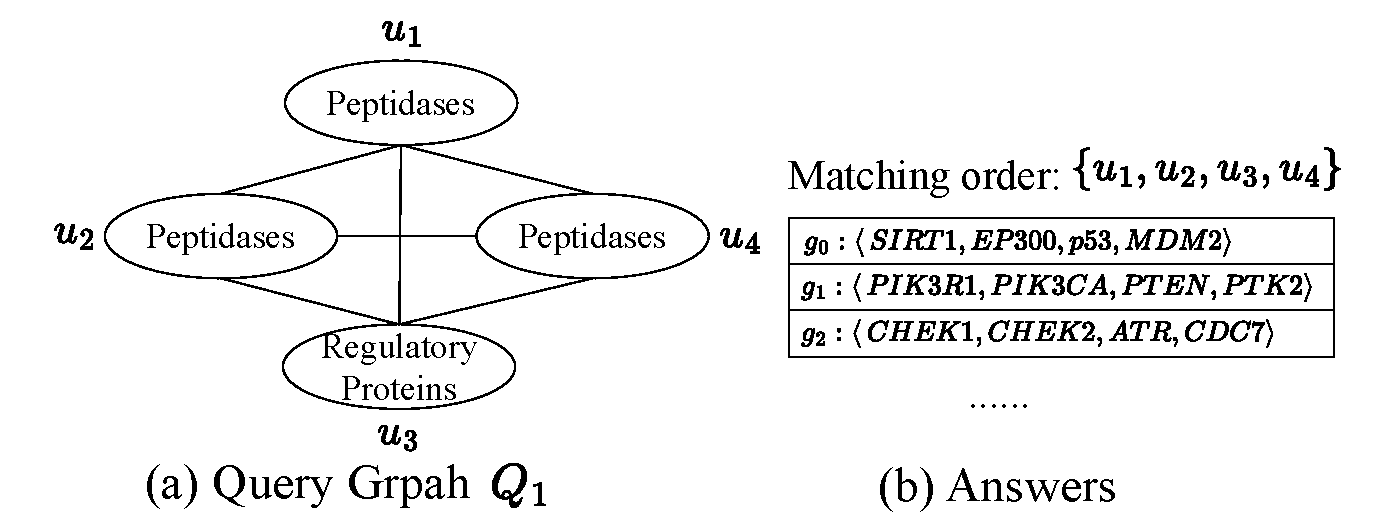
\includegraphics{./exp/newFIg/human_casestudy.pdf}
%     }
%     \caption{基于蛋白质相互作用网络的案例研究}
%     \label{fig:human-caseStudy}
%     \end{figure}    
% 图 \ref{fig:human-caseStudy} 展示了一个查询图 $Q_1$ 及其在蛋白质相互作用网络~\cite{dat-protein} 中的查询结果。
%     查询图$Q_1$ 表示由一个调节蛋白和3个肽酶组成的关键结构,边的权重表示它们之间的相互促进或抑制的程度。
%     我们根据边的权重优先级对子图进行排序,以识别与相互作用度最高的前 $k$ 个子图。
%     在匹配序列 $\{u_1, u_2, u_3, u_4\}$ 下,最密集的答案是 $g_0=$\{$SIRT1$, $EP300$, $p53$, $MDM2$\}。
%     值得注意的是,$p53$ 是在人类细胞中广泛研究的肿瘤抑制蛋白,而其他三个蛋白激酶表现出强烈的相互作用,并对 $p53$ 的活性产生显著的促进作用,这可能与肿瘤疾病的状态密切相关。
\section{本章小结}
本章详细介绍了我们提出的算法的实验设计与结果分析。
在实验设计部分,我们首先介绍了实验环境与配置。包括硬件和软件平台的详细信息、五个真实数据集、查询图的生成方式、以及参与测试的算法。
在实验过程中,我们通过从数据图中随机抽取子图生成查询图,并对不同查询图大小和不同的$k$值进行了全面测试。
接着,我们对实验结果进行深入分析,重点对比了不同算法在时间和空间效率方面的表现。实验结果表明,与现有的解决方案相比,我们提出的方案在插入与删除效率上表现出显著优势,性能提升达到2至4个数量级,验证了我们优化方法在处理大规模数据集时的有效性和优越性。

此外,我们对比了我们自己提出的四种不同的算法版本,分别是基线算法、全局MWstar算法、全局与局部MWstar结合的算法以及最终提出的压缩图上的MWstar算法。
实验结果表明,我们的最终算法显著优于基线方法,提升了$1\sim2$个数量级。同时,基于MWstar的全局和局部索引方法也表现出明显的性能优势,特别是在搜索效率方面,进一步证明了我们算法的有效性和优越性。
% 最后,我们还给出了CSM-TopK问题在蛋白质相互交互网络上的案例研究,验证了此算法的应用研究价值。